\documentclass[10pt, a4paper]{article}

% Formatting

\usepackage[utf8]{inputenc}
\usepackage[a4paper, top=1cm, left = 2cm, right = 2cm, bottom = 2cm]{geometry}
\usepackage[titletoc, title]{appendix}

\usepackage{amsmath, amsfonts, amssymb, mathtools}
\usepackage{graphicx, float}

\title{ESO207 Programming Assignment 1}
\author{Debaditya Bhattacharya}
\date{\today}

\begin{document}

\maketitle

\noindent\begin{minipage}{2in}
    \textbf{Name: }Debaditya Bhattacharya \\
    \textbf{Email id: }debbh@iitk.ac.in  
\end{minipage}
\hfill
\noindent\begin{minipage}{1.9in}
    \textbf{Roll No: }190254\\
    \textbf{Hackerrank Id: }debbh922
\end{minipage}

\noindent\rule{\textwidth}{1px}

\noindent\large{\textbf{Question 1 (a)}}
\vspace{5pt}

\noindent\normalsize Let $U(n)$ and $D(n)$ be the total possible localities directed "upwards" and "downwards"
respectively. We define the recurrence relation as follows:

\begin{align*}
    U(1) &= 3\\
    D(1) &= 1\\\\
    U(n) &= 3U(n-1) + D(n-1)\\
    D(n) &= U(n-1) + 3D(n-1)\\
\end{align*}
\vspace{-1.5cm}
\begin{align*}
    \forall n > 1, n \in \mathbb{N}
\end{align*}

\noindent\large{\textbf{Question 1 (e)}}

\begin{figure}[h]
    \centering
    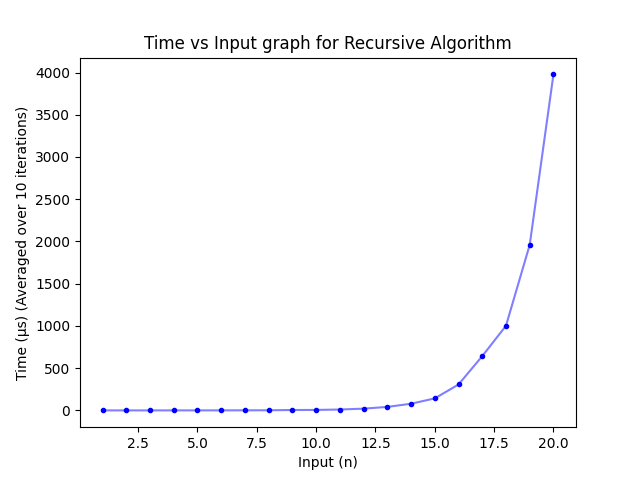
\includegraphics[width=15cm]{Recursive_Plot.png}
    \caption{Average runtime for recursive algorithm}
    \label{fig:m}
\end{figure}

\begin{figure}[h]
    \centering
    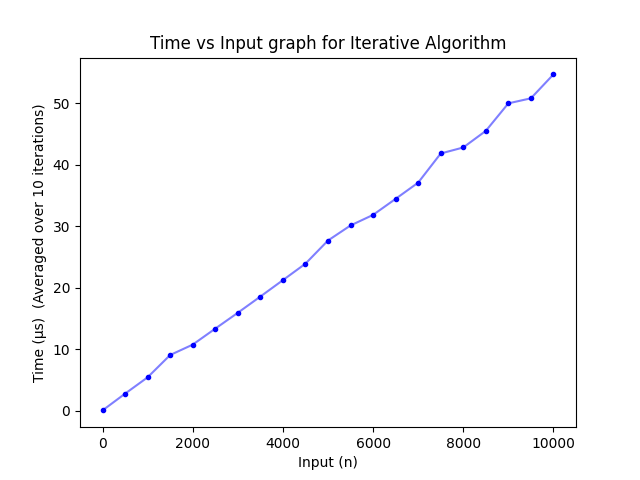
\includegraphics[width=15cm]{Iterative_Plot.png}
    \caption{Average runtime for iterative algorithm}
    \label{fig:m}
\end{figure}

\begin{figure}[h]
    \centering
    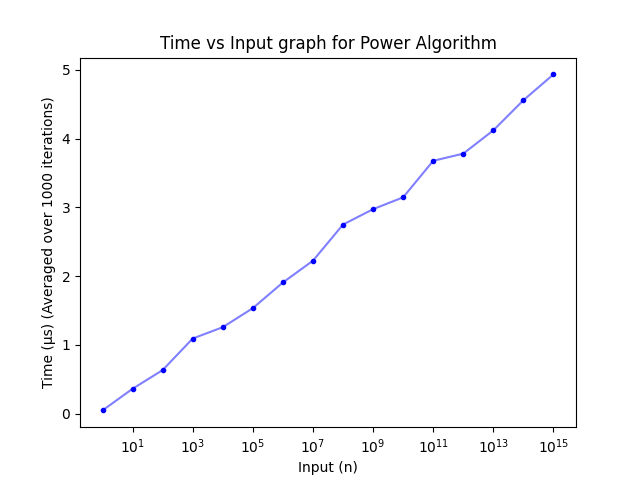
\includegraphics[width=15cm]{Power_Plot.png}
    \caption{Average runtime for power algorithm}
    \label{fig:m}
\end{figure}



\end{document}
